% file: rdt-research-spec.tex

\documentclass[tikz]{standalone}

\usetikzlibrary{mindmap, backgrounds, shapes, positioning, fit}

\begin{document}
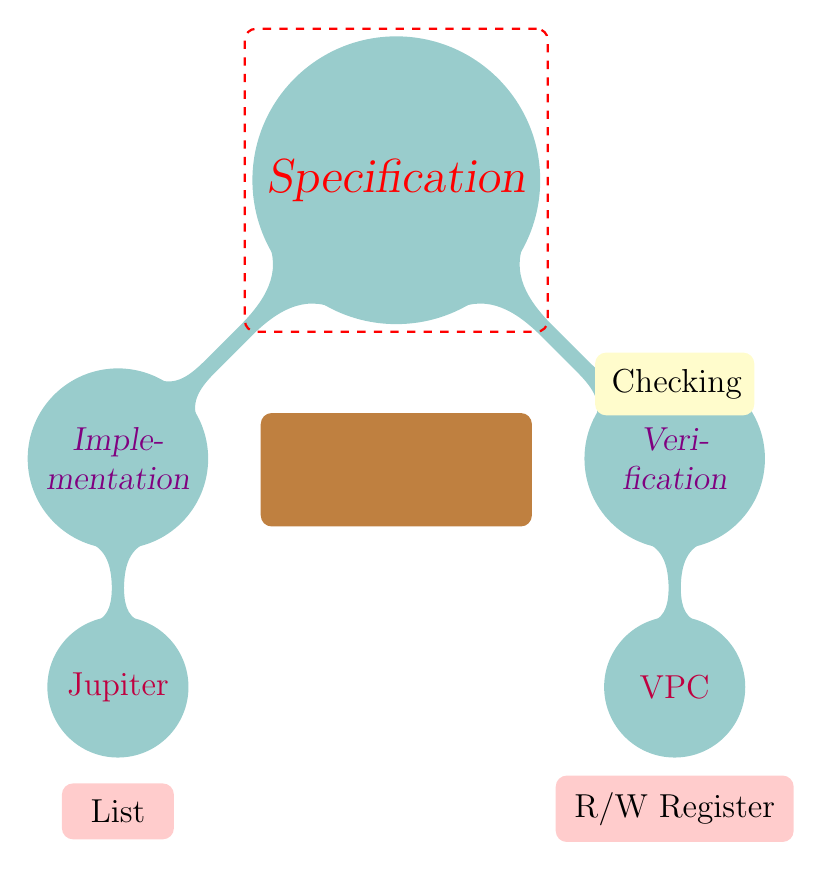
\begin{tikzpicture}[
    root concept/.append style = {concept color = teal!40, sibling angle = 90, font = \LARGE, minimum size = 0pt, red},
    level 1 concept/.append style = {concept color = teal!40, sibling angle = 90, font = \large, violet},
    level 2 concept/.append style = {concept color = teal!40, font = \large, purple},
    every annotation/.style = {fill = red!20, font = \sf, align = center, font = \large,
      minimum size = 5pt, inner sep = 6pt, text width = 2.6cm}
  ] 
  \path[mindmap]
    node (spec) [concept] {\textsl{Specification}}
    [counterclockwise from = 225]

    child[] {
      node (impl) [concept] {\textsl{Imple\-mentation}}
      [counterclockwise from = -90]
      child { node (jupiter) [concept, font = \large] {Jupiter} }
    }
    child[] {
      node (veri) [concept] {\textsl{Veri\-fication}}
      [clockwise from = -90]
      child { node (vpc) [concept, font = \large] {VPC} }
    };

    \node [annotation, fill = yellow!20, above = 0.40cm of veri.center, text width = 1.6cm] {Checking};
    \node (list) [annotation, below = 0.20cm of jupiter.south, text width = 1.0cm] {List};
    \node (reg) [annotation, below = 0.10cm of vpc.south] {R/W Register};

    \node [annotation, fill = brown!20, below = 1.00cm of spec.south, font = \Huge, inner sep = 12pt, brown] {RDT};

    \node () [draw, dashed, thick, red, rectangle, rounded corners, fit = (spec)] {};
\end{tikzpicture}
\end{document}

